\documentclass[reqno]{amsart}
\usepackage{enumerate}
\usepackage{amsmath}
\usepackage{scrextend}
\usepackage{bm}
\usepackage{algorithm}
\usepackage{algpseudocode}
\usepackage{graphicx}
\usepackage{enumitem}
\usepackage{tcolorbox}
\usepackage[headheight=12pt,textwidth=7in,top=1in, bottom=1in]{geometry}
\usepackage{listings}
\usepackage{cancel}
\usepackage{color} %red, green, blue, yellow, cyan, magenta, black, white
\definecolor{mygreen}{RGB}{28,172,0} % color values Red, Green, Blue
\definecolor{mylilas}{RGB}{170,55,241}

\usepackage[]{xcolor}
\definecolor{lightblue}{rgb}{0.63, 0.74, 0.78}
\definecolor{seagreen}{rgb}{0.18, 0.42, 0.41}
\definecolor{orange}{rgb}{0.85, 0.55, 0.13}
\definecolor{silver}{rgb}{0.69, 0.67, 0.66}
\definecolor{rust}{rgb}{0.72, 0.26, 0.06}
\definecolor{purp}{RGB}{68, 14, 156}

\colorlet{lightrust}{rust!50!white}
\colorlet{lightorange}{orange!25!white}
\colorlet{lightlightblue}{lightblue}
\colorlet{lightsilver}{silver!30!white}
\colorlet{darkorange}{orange!75!black}
\colorlet{darksilver}{silver!65!black}
\colorlet{darklightblue}{lightblue!65!black}
\colorlet{darkrust}{rust!85!black}
\colorlet{darkseagreen}{seagreen!85!black}

\usepackage{hyperref}
\hypersetup{
  colorlinks=true,
}

\hypersetup{
  linkcolor=darkrust,
  citecolor=seagreen,
  urlcolor=darkrust,
  pdfauthor=author,
}

\usepackage{cleveref}

%some custom commands you may find useful
\usepackage{xparse}
\DeclareDocumentCommand{\diff}{O{} m}{
	\frac{\mathrm{d} #1}{\mathrm{d}#2}
}
\DeclareDocumentCommand{\difftwo}{O{} m}{
	\frac{\mathrm{d}^2 #1}{\mathrm{d}#2^2}
}
\DeclareDocumentCommand{\pdiff}{O{} m}{
	\frac{\partial #1}{\partial #2}
}
\DeclareDocumentCommand{\pdifftwo}{O{} m}{
	\frac{\partial^{2} #1}{\partial #2^{2}}
}
\DeclareDocumentCommand{\integral}{O{} O{} m O{x}}{
	\int_{#1}^{#2} #3\ \mathrm{d}#4
}
\DeclareDocumentCommand{\sp}{}{
	\qquad \qquad \qquad }{
}
\NewDocumentEnvironment{solution}{}{
	\begin{addmargin}[2em]{0pt}
	}{\end{addmargin} \vskip0.25cm
}

\newenvironment{sysmatrix}[1]
{\left(\begin{array}{@{}#1@{}}}
	{\end{array}\right)}
\newcommand{\ro}[1]{%
	\xrightarrow{\mathmakebox[\rowidth]{#1}}%
}
\newlength{\rowidth}% row operation width
\AtBeginDocument{\setlength{\rowidth}{3em}}

\def\name{Ben Wilfong} %your name goes here
\def\ID{bwilfong3} %your cm goes here

%these packages create the footer and page numbering
\usepackage{fancyhdr}
\usepackage{lastpage}
\pagestyle{fancy}
\lhead{\name}
%%%%%%%%%%%%%%%%%%%%%%%%%%%%%%%%
\chead{ME 7751 Homework \#1}
%%%%%%%%%%%%%%%%%%%%%%%%%%%%%%%%
\rhead{Username: \ID}
\fancyfoot[C]{\footnotesize Page \thepage\ of \pageref{LastPage}}
\fancypagestyle{firststyle}
{ \renewcommand{\headrulewidth}{0pt}%
	\fancyhf{}%
	\fancyfoot[C]{\footnotesize Page \thepage\ of \pageref{LastPage}}
}

\lstset{frame=tb,
  language=[90]Fortran,
  aboveskip=3mm,
  belowskip=3mm,
  showstringspaces=false,
  columns=flexible,
  basicstyle={\footnotesize\ttfamily},
  numbers=none,
  numberstyle=\tiny\color{gray},
  keywordstyle=\color{darklightblue},
  commentstyle=\color{seagreen},
  stringstyle=\color{darkrust},
  breaklines=true,
  breakatwhitespace=true,
  tabsize=3,
}

\begin{document}
	\noindent
	\thispagestyle{firststyle}
	\begin{tabular}{l}
		{\LARGE \textbf{ME 7751: Intro to CFD} }\\
		%%%%%%%%%%%%%%%%%%%%%%%%%
		{\Large Homework Set \#1}
		%%%%%%%%%%%%%%%%%%%%%%%%%
	\end{tabular} \hfill \begin{tabular}{r}
		\name \\
		Username: \ID
	\end{tabular}
	\noindent\makebox[\linewidth]{\rule{\textwidth}{1pt}}

    \section{Part A - Numerical Method}
    \noindent The one dimensional steady state transport equation
    \begin{equation*}
        U\pdiff[\phi]{x} = \pdiff{x}\left(\Gamma \pdiff[\phi]{x}\right) + Q
    \end{equation*}
    can be discretized with central differences as
    \begin{equation}
        U\frac{\phi_{i + 1} - \phi_{i - 1}}{2\Delta x} - \underbrace{\frac{\left(\Gamma\pdiff[\phi]{x}\right)_{i + 1/2} - \left(\Gamma \pdiff[\phi]{x}\right)_{i - 1/2}}{\Delta x}}_{b} = Q_i.
    \label{eqn:a}
    \end{equation}
    The first derivatives in the numerator of $b$ can be written as
    \begin{equation}
        \left(\Gamma\pdiff[\phi]{x}\right)_{i + 1/2} = \Gamma_{i + 1/2}\frac{\phi_{i + 1} - \phi_{i}}{\Delta x}\quad \text{ and  }\quad \left(\Gamma\pdiff[\phi]{x}\right)_{i - 1/2} = \Gamma_{i - 1/2}\frac{\phi_{i} - \phi_{i-1}}{\Delta x}.
    \label{eqn:b}
    \end{equation}
    Substituting \cref{eqn:b} into \cref{eqn:a} and rearanging gives
    \begin{align}
    U\frac{\phi_{i + 1} - \phi_{i - 1}}{2\Delta x} -
    \frac{\Gamma_{i + 1/2}\frac{\phi_{i + 1} - \phi_{i}}{\Delta x} - \Gamma_{i - 1/2}\frac{\phi_{i} - \phi_{i - 1}}{\Delta x}}{\Delta x} & = Q_i \notag \\
    U\frac{\phi_{i + 1} - \phi_{i - 1}}{2\Delta x} -
    \frac{\Gamma_{i + 1/2}\phi_{i + 1} - (\Gamma_{i + 1/2} + \Gamma_{i - 1/2})\phi_{i} + \Gamma_{i - 1/2}\phi_{i -1}}{\left(\Delta x\right)^2} &= Q_i \notag \\
    \left(\frac{U}{2\Delta x} - \frac{\Gamma_{i + 1/2}}{(\Delta x)^2}\right)\phi_{i + 1} +
    \left(\frac{\Gamma_{i + 1/2} + \Gamma_{i - 1/2}}{(\Delta x)^2}\right)\phi_i -
    \left(\frac{U}{2\Delta x} + \frac{\Gamma_{i - 1/2}}{(\Delta x)^2}\right)\phi_{i - 1} &= Q_i \label{eqn:c}.
    \end{align}
    \Cref{eqn:c} can be cast as the system of linear equations
    \begin{equation*}
        \underbrace{\begin{bmatrix}
        1 \\
        -\left(\frac{U}{2\Delta x} + \frac{\Gamma_{1/2}}{(\Delta x)^2}\right) & \frac{\Gamma_{3/2}+\Gamma_{1/2}}{(\Delta x)^2} & \frac{U}{2\Delta x} - \frac{\Gamma_{3/2}}{(\Delta x)^2} \\
        \ddots & \ddots & \ddots \\
        & -\left(\frac{U}{2\Delta x} + \frac{\Gamma_{N - 3/2}}{(\Delta x)^2}\right) & \frac{\Gamma_{N - 1/2}+\Gamma_{N - 3/2}}{(\Delta x)^2} & \frac{U}{2\Delta x} - \frac{\Gamma_{i -1/2}}{(\Delta x)^2} \\
        &&& 1
\end{bmatrix}}_{\mathrm{\bm{A}}}
\underbrace{\begin{pmatrix} \phi_{0} \\ \phi_{1} \\ \vdots \\ \phi_{N-1} \\ \phi_{N} \end{pmatrix}}_{\Phi}
        =
        \underbrace{\begin{pmatrix} 1 \\ Q_1 \\ \vdots \\ Q_{N-1} \\ 0 \end{pmatrix}}_{b}
    \end{equation*}
    for a discretization at $\{x_0,\ x_1,\ \dots \, x_N\} = \{0,\ \Delta x,\ 2\Delta x,\dots,\ N\Delta x$\}.
    The boundary conditions are given by $\phi_{-1/2} = 1$ and $\phi_{N + 1/2} = 0$. \\~\\
    For the cases in which $U,\ \Gamma,$ and $Q$ are constant, the solution is found via the following steps:
    \begin{enumerate}
        \item Populate the matrix $\mathrm{\bm{A}}$
        \item Populate the vector $b$
        \item Solve $A\Phi = b$ for the vector $\Phi$ using TDMA
    \end{enumerate}
    When $U,\ \Gamma,$ or $Q$ depend on the value of $\phi$ the problem becomes nonlinear and an iterative approach must be taken.
    For nonlinear problems, the solution is found via the following steps:
    \begin{enumerate}
        \item Make an initial guess for the vector $\Phi^{(0)}$
        \item Calculate $U(\Phi^{(n)}),\ \Gamma(\Phi^{(n)}),$ and $Q(\Phi^{(n)})$
        \item Populate the matrix $A$
        \item Populate the vector $b$
        \item Solve $A\Phi^{(n+1)} = b$ for the vector $\Phi^{(n+1)}$ using TDMA
        \item Repeat steps 2 though 5 until convergence
    \end{enumerate}
    For this problem I will use a discretization of $\phi(x) = 1 - x/L$ as an initial guess. \\~\

    \noindent The tridiagonal matrix $A$ is stored in an $N+1\times 3$ to take advantage of it's sparsity.
    The lower, center, and upper diagonal are stored in $A_{1:N,0}$, $A_{0:N,1}$, and $A_{0:N-1,2}$.
    The tridiagonal linear solve using this data structure is given in \cref{alg:TDMA}. \\ \vspace{-0.25in}
    \begin{center}\begin{minipage}{0.5\textwidth}\begin{algorithm}[H]
        \caption{Tridiagonal Matrix Algorithm} \label{alg:TDMA}
        \begin{algorithmic}
            \State Given: $A$ \Comment{$N+1\times N+1$}
            \State Given: $x$ \Comment{$N+1\times 1$}
            \State Given: $b$ \Comment{$N+1\times 1$}
            \State
            \For{$i = 1:N$} \Comment{In place LU factorization}
                \State $w = A_{i,0}/A_{i-1,1}$
                \State $A_{i,0} = A_{i,0} - wA_{i-1,1}$
                \State $A_{i,1} = A_{i,0} - wA_{i-1,2}$
                \State $A_{i,0} = w$
            \EndFor
            \State
            \State $y_0 = b_0$ \Comment{Forward Substitution}
            \For{$i = 1:N$}
                \State $y_i = b_i - A_{i,0)y_{i - 1}}$
            \EndFor
            \State
            \State $x_N = y_N/A_{N,1}$ \Comment{Backward Substitution}
            \For{$i = N-1:-1:0$}
            \State $x_i = \frac{y_i - A_{i,2}x_{i + 1}}{A_{i,1}}$
            \EndFor
        \end{algorithmic}
    \end{algorithm}\end{minipage}\end{center}
    \section{Part B - Linear Problems}
    \Cref{fig:B} shows the solution, average error, and runtime for the case $U = 1,\ \Gamma = 0.1,$ and $Q = 0$ with $N = 10,\ 20,\ 30,\ 40,\ 50.$
    The error decreases with increasing $N$ as expected.
    The plot of average error versus $N$ shows that the method is second-order-accurate.
    This is because the error decreases with a slope of two in loglog space.
    This order of accuracy is expected given that central differences were used to discretize the derivatives.
    \begin{figure}
        \centering
        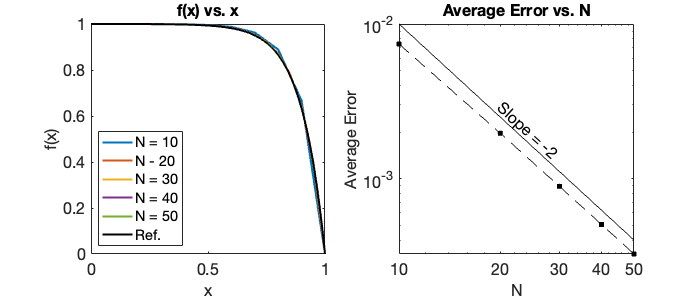
\includegraphics[width=4in]{partA.png}
        \caption{Solution and average error for $N = 10, 20, 30, 40, 50$}
        \label{fig:B}
    \end{figure}

    \section{Part C - Non-linear Problems}

\end{document}

